% PTE Core 模考 2B —— 口语 错题与详解·整理卷  版本 000（自包含）
% 编译: xelatex 本文件.tex   （需 Noto CJK + TeX Gyre Heros 字体）
% 本版本含图片，依赖同目录的 img/ 子目录。
\documentclass[11pt]{article}

% --------- 样式（原 ptestyle.sty，已内联）---------
% ============================================================
%  ptestyle.sty  —  PTE 模考错题整理卷 共享样式
%  编译引擎: XeLaTeX  (中英混排, 需要 Noto CJK 字体)
% ============================================================

\usepackage[a4paper,margin=2cm,headsep=4mm]{geometry}
\usepackage{fontspec}
\usepackage{xeCJK}
\usepackage[table]{xcolor}
\usepackage[normalem]{ulem}        % \sout 删除线
\usepackage{tabularx}
\usepackage{array}
\usepackage{ragged2e}
\usepackage{enumitem}
\usepackage[most]{tcolorbox}
\usepackage{fancyhdr}
\usepackage{graphicx}
\usepackage{pifont}                % \ding{51}=✓ \ding{55}=✗（阅读对错标注）
\usepackage{needspace}
\usepackage{tikz}

% ---------- 字体 ----------
\setmainfont{TeX Gyre Heros}            % 拉丁: Helvetica 风格(纤细清晰)
\setCJKmainfont{Noto Sans CJK SC}
\setCJKsansfont{Noto Sans CJK SC}
\newfontfamily\cjkserif{Noto Serif CJK SC}
\linespread{1.18}
\setlength{\parindent}{0pt}
\setlength{\parskip}{4pt}

% ---------- 配色 ----------
\definecolor{cWrong}{HTML}{D32F2F}     % 红  = 修改 / 错误
\definecolor{cFix}{HTML}{1B7F3B}       % 绿  = 正确建议
\definecolor{cDelete}{HTML}{1565C0}    % 蓝  = 删除
\definecolor{cInsert}{HTML}{7B1FA2}    % 紫  = 插入
\definecolor{cPartial}{HTML}{E07B00}   % 橙  = 部分得分
\definecolor{cNote}{HTML}{0277BD}      % 蓝  = 注解
\definecolor{cAccent}{HTML}{16A085}    % 主题青绿(平台主色)
\definecolor{cWrongBg}{HTML}{FBE0E0}
\definecolor{cDelBg}{HTML}{DCE8FB}
\definecolor{cInsBg}{HTML}{EEE0F5}
\definecolor{cHead}{HTML}{20303A}
\definecolor{cGrayBox}{HTML}{F4F6F7}
\definecolor{cModelBg}{HTML}{EAF7EF}
\definecolor{cYouBg}{HTML}{FFF7F5}
\definecolor{cNoteBg}{HTML}{EAF3FA}
\definecolor{cRule}{HTML}{D7DEE2}

% ---------- 行内批改宏 (复刻平台标注) ----------
% \fix{原词}{正确}  红色删除线 + 绿色上标改正  (修改/拼写/空格)
\newcommand{\fix}[2]{%
  \colorbox{cWrongBg}{\textcolor{cWrong}{\sout{#1}}}%
  \,\textsuperscript{\textcolor{cFix}{\footnotesize #2}}}
% \del{原词}  蓝色删除线  (应删除)
\newcommand{\del}[1]{%
  \colorbox{cDelBg}{\textcolor{cDelete}{\sout{#1}}}%
  \,\textsuperscript{\textcolor{cDelete}{\footnotesize 删}}}
% \ins{词}  紫色下划线  (应插入)
\newcommand{\ins}[1]{%
  \textsuperscript{\textcolor{cInsert}{\footnotesize $\wedge$}}%
  \colorbox{cInsBg}{\textcolor{cInsert}{#1}}}
% \miss{词}  灰色删除线  (口语漏读 / 未作答)
\newcommand{\miss}[1]{\textcolor{gray}{\sout{#1}}}
% \add{原词}{改正}  橙色波浪线 + "补"标签  (平台漏标、本卷补标的错误)
\definecolor{cAdd}{HTML}{E65100}
\newcommand{\add}[2]{%
  \textcolor{cAdd}{\uwave{#1}}%
  \,\textsuperscript{\textcolor{cAdd}{\footnotesize 补：#2}}}
% 高亮(口语发音): 好/中/差
\newcommand{\spk}[2]{\textcolor{#1}{#2}}

% ---------- 评分单元格着色 ----------
\newcommand{\sfull}[1]{\textcolor{cFix}{\bfseries #1}}     % 满分
\newcommand{\spart}[1]{\textcolor{cPartial}{\bfseries #1}} % 部分
\newcommand{\szero}[1]{\textcolor{cWrong}{\bfseries #1}}   % 零/低分

% ---------- 分数小标签 ----------
\newtcbox{\chip}[1][cAccent]{on line, boxsep=2pt, left=4pt, right=4pt, top=1pt,
  bottom=1pt, arc=3pt, colback=#1, colframe=#1, coltext=white, nobeforeafter,
  fontupper=\bfseries\footnotesize}

% ---------- 题块小标题 ----------
\newcommand{\ptesub}[1]{%
  \par\needspace{2\baselineskip}\smallskip
  {\color{cAccent}\rule[-0.2ex]{3pt}{1.05em}}\hspace{6pt}%
  {\bfseries\color{cHead}#1}\par\nopagebreak\smallskip}

% ---------- 题块外框 ----------
% \begin{qblock}{标号·题型}{右上信息(得分/用时)} ... \end{qblock}
\newtcolorbox{qblock}[2]{
  breakable, enhanced, arc=2.5pt,
  colback=white, colframe=cRule, boxrule=0.6pt,
  left=11pt, right=11pt, top=8pt, bottom=10pt,
  toptitle=3pt, bottomtitle=3pt, lefttitle=11pt, righttitle=11pt,
  colbacktitle=cHead, coltitle=white, fonttitle=\bfseries,
  title={#1\hfill\normalfont\bfseries\small #2}}

% ---------- 文本块: 题干 / 范文 / 你的作答 / 建议 ----------
\newtcolorbox{promptbox}{enhanced, breakable, colback=cGrayBox, colframe=cGrayBox,
  arc=2pt, left=8pt, right=8pt, top=6pt, bottom=6pt, boxrule=0pt}
\newtcolorbox{modelbox}{enhanced, breakable, colback=cModelBg, colframe=cModelBg,
  borderline west={3pt}{0pt}{cFix}, arc=1pt, left=8pt, right=8pt, top=6pt, bottom=6pt, boxrule=0pt}
\newtcolorbox{youbox}{enhanced, breakable, colback=cYouBg, colframe=cYouBg,
  borderline west={3pt}{0pt}{cWrong}, arc=1pt, left=8pt, right=8pt, top=6pt, bottom=6pt, boxrule=0pt}
\newtcolorbox{notebox}{enhanced, breakable, colback=cNoteBg, colframe=cNoteBg,
  borderline west={3pt}{0pt}{cNote}, arc=1pt, left=8pt, right=8pt, top=6pt, bottom=6pt, boxrule=0pt}

% ---------- 评分表 ----------
% 用法见正文; 这里给表头宏
\newcommand{\scorehead}{%
  \rowcolors{2}{cGrayBox}{white}
  \arrayrulecolor{cRule}}

% ---------- 章节大标题 ----------
\newcommand{\ptesection}[3]{% #1=中文名 #2=英文名 #3=该项分数
  \addcontentsline{toc}{section}{#1}%
  \needspace{6\baselineskip}
  \begin{tcolorbox}[enhanced, colback=cAccent, colframe=cAccent, sharp corners,
     left=14pt, right=14pt, top=10pt, bottom=10pt, boxrule=0pt]
    {\fontsize{20}{24}\selectfont\bfseries\color{white} #1\ \ }%
    {\large\color{white!85} #2}\hfill
    {\large\color{white}本项得分\ \ }{\fontsize{22}{24}\selectfont\bfseries\color{white} #3}%
    \ {\color{white!85}/ 90}
  \end{tcolorbox}}

% ---------- 题型小节分隔 (口语 RA/RS/DI/RTS/ASQ 等) ----------
\newcommand{\ptetask}[2]{%
  \addcontentsline{toc}{subsection}{#1\ #2}%
  \needspace{4\baselineskip}\medskip
  \begin{tcolorbox}[enhanced, colback=cHead, colframe=cHead, sharp corners,
     left=12pt, right=12pt, top=5pt, bottom=5pt, boxrule=0pt]
    {\large\bfseries\color{white} #1}\ \ {\color{white!80} #2}
  \end{tcolorbox}\smallskip}

% ---------- 口语 AI 语音识别着色 (复刻平台: 优/良/差 + 停顿) ----------
\definecolor{cSpkGood}{HTML}{2E9E5B}   % 优 绿
\definecolor{cSpkOk}{HTML}{C77F00}     % 良 黄/琥珀
\definecolor{cSpkBad}{HTML}{E0352B}    % 差 红
\newcommand{\sg}[1]{\textcolor{cSpkGood}{#1}}   % 优
\newcommand{\sy}[1]{\textcolor{cSpkOk}{#1}}     % 良
\newcommand{\sr}[1]{\textcolor{cSpkBad}{#1}}    % 差
\newcommand{\smiss}[1]{\textcolor{cSpkBad}{\sout{#1}}}  % 漏读 (红删除线)
\newcommand{\pse}{{\color{gray}\,/\,}}          % 停顿
\newcommand{\asrlegend}{{\footnotesize\color{gray}AI 语音识别\quad
  {\color{cSpkGood}\textbullet}\,优\ \ {\color{cSpkOk}\textbullet}\,良\ \
  {\color{cSpkBad}\textbullet}\,差\ \ {\color{gray}/}\,停顿\ \
  {\color{cSpkBad}\sout{词}}\,漏读}}
\newtcolorbox{asrbox}{enhanced, breakable, colback=white, colframe=cRule,
  boxrule=0.6pt, arc=1pt, left=8pt, right=8pt, top=6pt, bottom=6pt}

% ---------- 中文翻译行 ----------
\newcommand{\zh}[1]{{\footnotesize\textcolor{cNote}{\textbf{译}}\ \textcolor{gray}{#1}}}

% ---------- 阅读填空 / 选择 对错标注 ----------
\newcommand{\rok}[1]{{\color{cFix}\ding{51}\,#1}}                 % 选对(绿勾 + 词)
\newcommand{\rno}[2]{{\color{cWrong}\ding{55}\,\sout{#1}}\,{\footnotesize\color{cFix}(答案:\,#2)}}  % 选错: 你的(红删) + (答案:正确)
\newcommand{\rblank}[1]{{\color{cFix}\underline{\,#1\,}}}         % 直接给空的正确答案(无你的作答时)

% ---------- 听力专用 ----------
\newcommand{\hiw}[2]{{\color{cWrong}\uline{#1}}\,{\footnotesize\color{cFix}(听:#2)}} % HIW: 屏幕错词(红下划线)+ 实际读音
\newcommand{\lhit}[1]{{\color{cFix}#1}}                           % WFD: 命中的词(绿)
\newcommand{\lmiss}[1]{{\color{cWrong}\sout{#1}}}                 % WFD: 多余/错误的词(红删, 1B 配色)
% ---- WFD 逐词批改 · 本套 2B 平台配色（与 1B 相反）：绿=命中 / 红括号=漏写 / 灰删除线=多写或听错 ----
% 说明: 2B 平台把"漏写"标红(加括号)、"多写/听错"标灰删除线; 本卷忠于原图按此复刻。
\newcommand{\womit}[1]{{\color{cWrong}(#1)}}                      % WFD: 漏写(正确答案有、你没写)——红色括号
\newcommand{\wbad}[1]{{\color{gray}\sout{#1}}}                    % WFD: 多写/听错(你写了但错)——灰删除线
\newcommand{\wfdlegend}{{\footnotesize\color{gray}WFD 配色：\
  {\color{cFix}命中}\ \ {\color{cWrong}(漏写)}\ \ {\color{gray}\sout{多写/听错}}}}

% ---------- 颜色图例 ----------
\newcommand{\ptelegend}{%
  \begin{tcolorbox}[enhanced, colback=cGrayBox, colframe=cRule, boxrule=0.5pt,
    arc=2pt, left=10pt, right=10pt, top=6pt, bottom=6pt]
  {\bfseries\color{cHead}颜色说明\quad}
  \fix{改}{正}~修改/拼写\quad
  \del{删}~应删除\quad
  \ins{插}~应插入\quad
  \add{补}{改正}~平台漏标(本卷补标)\quad
  {\color{cFix}\rule{1em}{0.6em}}~范文/正确\quad
  {\color{cNote}\rule{1em}{0.6em}}~AI 建议
  \end{tcolorbox}}

% ---------- 页眉页脚 ----------
\pagestyle{fancy}
\fancyhf{}
\renewcommand{\headrulewidth}{0.4pt}
\renewcommand{\footrulewidth}{0pt}
\fancyhead[L]{\footnotesize\color{cHead}\bfseries PTE Core 模考 2B}
\fancyhead[R]{\footnotesize\color{gray} 错题与详解整理卷}
\fancyfoot[C]{\footnotesize\color{gray}\thepage}

\begin{document}

% --------- 封面（原 cover.tex）---------
% ---------- 封面 / 成绩总览 ----------
\definecolor{mListen}{HTML}{1F3A5F}
\definecolor{mRead}{HTML}{C2D70B}
\definecolor{mSpeak}{HTML}{4D4D4D}
\definecolor{mWrite}{HTML}{A01B7D}

\begin{titlepage}
\thispagestyle{empty}
\centering
\vspace*{1.4cm}

{\fontsize{30}{36}\selectfont\bfseries\color{cHead} PTE Core 模考 2B}\\[4mm]
{\fontsize{17}{20}\selectfont\color{cAccent}\bfseries 错题与详解 · 整理卷}\\[3mm]
{\color{gray} APEUni / 猩际 PTE 模考　·　提交时间 2026-06-28 11:49}\\[1.2cm]

% ---- 总分 ----
\begin{tcolorbox}[width=0.62\textwidth, halign=center, enhanced,
  colback=cAccent, colframe=cAccent, arc=6pt, boxrule=0pt, top=10pt, bottom=10pt]
  {\color{white}\large 总分 Overall}\\[2pt]
  {\fontsize{46}{50}\selectfont\bfseries\color{white} 50}
\end{tcolorbox}

\vspace{1.0cm}

% ---- 四项分数条形图 ----
\begin{tcolorbox}[width=0.84\textwidth, enhanced, colback=white, colframe=cRule,
  boxrule=0.8pt, arc=4pt, left=18pt, right=18pt, top=14pt, bottom=14pt]
\setlength{\tabcolsep}{6pt}\renewcommand{\arraystretch}{1.7}
\sffamily
\begin{tabular}{@{}r@{\hskip 8pt}l@{\hskip 10pt}l@{}}
 \bfseries Listening 听力 & {\color{mListen}\rule{5.22cm}{0.42cm}} & {\bfseries\large 47}\\
 \bfseries Reading 阅读   & {\color{mRead}\rule{5.11cm}{0.42cm}}   & {\bfseries\large 46}\\
 \bfseries Speaking 口语  & {\color{mSpeak}\rule{4.00cm}{0.42cm}}  & {\bfseries\large 36}\\
 \bfseries Writing 写作   & {\color{mWrite}\rule{7.89cm}{0.42cm}}  & {\bfseries\large 71}\\
\end{tabular}\\[2mm]
{\footnotesize\color{gray} 满分 90　|　刻度: 条长 = 得分 / 90}
\end{tcolorbox}

\vfill
\begin{flushleft}\small\color{gray}
\textbf{说明:}本卷由本次模考的题目与"详解"截图逐题誊写、重新排版而成,完整保留每道题的
\emph{题干 / 原文、范文、你的作答、逐项评分、彩色批改与 AI 中文建议}。\\
所有错误按平台标注用颜色标出(见下方图例)。原始"详解"PDF 不可复制、仅截图,本卷内容均为人工对照誊录,若与原图有出入以原图为准。
\end{flushleft}
\vspace{4mm}
\ptelegend
\end{titlepage}

% --------- 口语正文（原 sec_speaking_body.tex）---------
% ===================== 口语 Speaking =====================
\ptesection{口语}{Speaking · 5 题型}{36}

\vspace{1mm}
{\small\color{gray} 本部分共 \textbf{30 题}：\textbf{RA 朗读}Q1--7、\textbf{RS 复述句子}Q8--18、\textbf{DI 描述图}Q19--21、\textbf{RTS 情景应答}Q22--24、\textbf{ASQ 简短回答}Q25--30。每题保留\textbf{正确文本／范文}、\textbf{你的作答（AI 语音识别逐词配色）}与平台\textbf{逐项评分}，并附\textbf{中文翻译}。平台「AI 语音识别」按发音质量\textbf{逐词上色}，本卷逐词复刻。RA／RS 的上色对象是\textbf{原文／原句}；DI／RTS 的上色对象是\textbf{你说出的话（语音识别原文，含口误照原样保留）}。
本套口语总分 \textbf{36 / 90}：发音、流利度普遍偏低是主要失分点。}

\vspace{1mm}
{\small\color{gray}\textbf{配色图例：}\asrlegend}
\vspace{2mm}


\ptetask{朗读}{Read Aloud · RA　Q1--7（内容均 5/5，失分在发音／流利度）}
% ---------------- Q1 ----------------
\begin{qblock}{Q1\quad RA \#755\ \ Roman Army}{朗读 · 总分 \textcolor{cAccent}{\bfseries 18}/90}
\ptesub{原文 Text（朗读对象）}
\begin{promptbox}
There were two types of soldier in the Roman Army: the roman legionary and the auxiliaries. The legionaries were the very best soldiers and the auxiliaries were actually non-Roman citizens. Legionaries wore an undershirt made of linen and a woollen tunic. The linen helped the soldiers to stay cool while the wool helped to trap heat, keeping the soldiers warm.
\end{promptbox}
\zh{罗马军队中有两类士兵：罗马军团士兵和辅助兵。军团士兵是最精锐的士兵，而辅助兵实际上是非罗马公民。军团士兵穿着亚麻制的内衣和羊毛束腰外衣。亚麻帮助士兵保持凉爽，而羊毛则有助于锁住热量、使士兵保暖。}
\ptesub{你的朗读（AI 语音识别逐词配色）}
\asrlegend
\begin{asrbox}
\sg{There} \sg{were} \sy{two} \sg{types} \sg{of} \pse \sr{soldier} \sg{in} \sg{the} \sg{Roman} \sg{Army} \pse \sg{the} \sr{roman} \sg{legionary} \sg{and} \sg{the} \sg{auxiliaries} \sg{The} \sg{legionaries} \sg{were} \sg{the} \pse \sg{very} \sg{best} \sg{soldiers} \sg{and} \sg{the} \sr{were} \sr{auxiliaries} \sg{were} \pse \sy{actually} \sr{non} \sr{Roman} \sr{citizens} \sr{Legionaries} \sg{wore} \sy{an} \sg{undershirt} \sg{made} \sg{of} \sg{linen} \sy{and} \sy{a} \sr{woollen} \sr{tunic} \sr{The} \sg{linen} \sg{helped} \sg{the} \pse \sg{soldiers} \sy{to} \sg{stay} \sg{cool} \sy{while} \sg{the} \sg{wool} \sy{helped} \sg{to} \sg{trap} \sy{heat} \pse \sr{keeping} \sg{the} \sg{soldiers} \sg{warm}
\end{asrbox}
\smallskip
{\small\textbf{评分：}内容 \sfull{5/5} \quad\textperiodcentered\quad 发音 \spart{21/90} \quad\textperiodcentered\quad 流利度 \szero{14/90}}\quad{\footnotesize\color{gray}（用时 01:08）}
\end{qblock}

% ---------------- Q2 ----------------
\begin{qblock}{Q2\quad RA \#715\ \ Mutual Politics}{朗读 · 总分 \textcolor{cAccent}{\bfseries 29}/90}
\ptesub{原文 Text（朗读对象）}
\begin{promptbox}
In order to achieve the free flow of goods and services, with work and capital between the member countries, they needed to establish mutual politics in areas as diverse as agriculture, transport, and when they were concerned with a far wider range of issues.
\end{promptbox}
\zh{为了实现商品和服务的自由流动，以及成员国之间劳动力与资本的自由流动，他们需要在农业、交通等诸多不同领域制定共同政策，而且他们所关注的议题范围要广泛得多。}
\ptesub{你的朗读（AI 语音识别逐词配色）}
\asrlegend
\begin{asrbox}
\sg{In} \sg{order} \sg{to} \sg{achieve} \sg{the} \sg{free} \sg{flow} \sg{of} \sy{goods} \sg{and} \sg{services} \pse \sg{with} \sg{work} \sg{and} \sg{capital} \pse \sg{between} \sg{the} \sg{member} \sg{countries} \pse \sg{they} \sg{needed} \sg{to} \sg{establish} \sg{mutual} \sy{politics} \pse \sg{in} \sg{areas} \sg{as} \sg{diverse} \sg{as} \sg{agriculture} \pse \sy{transport} \sg{and} \sg{when} \sg{they} \sg{were} \sg{concerned} \sg{with} \sy{a} \sg{far} \sg{wider} \sg{range} \sg{of} \sy{issues}
\end{asrbox}
\smallskip
{\small\textbf{评分：}内容 \sfull{5/5} \quad\textperiodcentered\quad 发音 \spart{31/90} \quad\textperiodcentered\quad 流利度 \spart{26/90}}\quad{\footnotesize\color{gray}（用时 00:59）}
\end{qblock}

% ---------------- Q3 ----------------
\begin{qblock}{Q3\quad RA \#377\ \ Mature Tree}{朗读 · 总分 \textcolor{cAccent}{\bfseries 25}/90}
\ptesub{原文 Text（朗读对象）}
\begin{promptbox}
The wonderful framework of mature trees creates a secluded, enclosed atmosphere that unites a great variety of plantings to inspire visitors in all seasons. Spring in the garden is marked by leafing up and flowering of trees and the eruption of the flowers in the bulb meadows, and woodland understory.
\end{promptbox}
\zh{成熟树木所构成的美妙框架营造出一种幽静、封闭的氛围，将种类繁多的植物联结在一起，在四季都能给游客以启迪。花园里的春天以树木抽叶开花、以及球根草甸与林下植被中花朵的绽放为标志。}
\ptesub{你的朗读（AI 语音识别逐词配色）}
\asrlegend
\begin{asrbox}
\sg{The} \sg{wonderful} \sg{framework} \sg{of} \sg{mature} \sy{trees} \sg{creates} \sg{a} \sr{secluded} \pse \sy{enclosed} \sg{atmosphere} \sg{that} \sg{unites} \sg{a} \pse \sg{great} \sg{variety} \sg{of} \pse \sg{plantings} \sg{to} \sg{inspire} \sg{visitors} \sg{in} \sg{all} \sg{seasons} \sg{Spring} \sg{in} \sg{the} \sg{garden} \sg{is} \sg{marked} \sg{by} \pse \sg{leafing} \sg{up} \sg{and} \sg{flowering} \sg{of} \pse \sg{trees} \sg{and} \sg{the} \sy{eruption} \sg{of} \sg{the} \sg{flowers} \sg{in} \sg{the} \sy{bulb} \sy{meadows} \pse \sg{and} \sg{woodland} \sg{and} \pse \sy{understory}
\end{asrbox}
\smallskip
{\small\textbf{评分：}内容 \sfull{5/5} \quad\textperiodcentered\quad 发音 \spart{28/90} \quad\textperiodcentered\quad 流利度 \spart{21/90}}\quad{\footnotesize\color{gray}（用时 01:07）}
\end{qblock}

% ---------------- Q4 ----------------
\begin{qblock}{Q4\quad RA \#710\ \ Antarctic}{朗读 · 总分 \textcolor{cAccent}{\bfseries 23}/90}
\ptesub{原文 Text（朗读对象）}
\begin{promptbox}
The world's fifth largest continent: Antarctica is almost entirely covered by ice 2000 meters thick. The area sustains varied wildlife including seals, whales, and penguins. The Antarctic treaty signed in 1959 and enforced since 1961 provides for international governance of Antarctica.
\end{promptbox}
\zh{世界第五大洲——南极洲几乎完全被 2000 米厚的冰层覆盖。该地区养育着包括海豹、鲸鱼和企鹅在内的多种野生动物。1959 年签署、1961 年起生效的《南极条约》规定了对南极洲的国际治理。}
\ptesub{你的朗读（AI 语音识别逐词配色）}
\asrlegend
\begin{asrbox}
\sg{The} \sg{world's} \sg{fifth} \sg{largest} \sy{continent} \pse \sr{Antarctica} \sg{is} \sg{almost} \sg{entirely} \sg{covered} \sg{by} \sr{ice} \sg{2000} \sg{meters} \sg{thick} \sy{The} \sg{area} \sg{sustains} \sg{varied} \pse \sy{wildlife} \pse \sg{including} \sy{seals} \pse \sy{whales} \sg{and} \sg{penguins} \sr{The} \sr{Antarctic} \sg{treaty} \sg{signed} \sg{in} \sg{1959} \sg{and} \sg{enforced} \sy{since} \sg{1961} \sg{provides} \sg{for} \pse \sg{international} \sg{governance} \sg{of} \sg{Antarctica}
\end{asrbox}
\smallskip
{\small\textbf{评分：}内容 \sfull{5/5} \quad\textperiodcentered\quad 发音 \spart{23/90} \quad\textperiodcentered\quad 流利度 \spart{22/90}}\quad{\footnotesize\color{gray}（用时 01:06）}
\end{qblock}

% ---------------- Q5 ----------------
\begin{qblock}{Q5\quad RA \#712\ \ Undergraduates Education}{朗读 · 总分 \textcolor{cAccent}{\bfseries 24}/90}
\ptesub{原文 Text（朗读对象）}
\begin{promptbox}
Undergraduates may choose to major in any one of 125 academic majors. The university's distinguished faculty includes internationally known scientists, authors and teachers who are committed to continuing the university's tradition in providing one of the highest quality undergraduate educations available.
\end{promptbox}
\zh{本科生可以从 125 个学术专业中任选其一作为主修。该校声名卓著的师资包括享誉国际的科学家、作家和教师，他们致力于延续学校的传统——提供现有最高质量的本科教育之一。}
\ptesub{你的朗读（AI 语音识别逐词配色）}
\asrlegend
\begin{asrbox}
\sy{Undergraduates} \sg{may} \sg{choose} \sg{to} \sg{major} \sg{in} \sg{any} \sg{one} \sg{of} \sg{125} \sg{academic} \sg{majors} \sg{The} \sg{university's} \sy{distinguished} \pse \pse \sr{faculty} \sg{includes} \sg{internationally} \sy{known} \sg{scientists} \pse \sg{authors} \sg{and} \sg{teachers} \sg{who} \sg{are} \sg{committed} \sg{to} \sy{continuing} \sg{the} \pse \sg{university's} \sg{tradition} \sg{in} \sg{providing} \sg{one} \sg{of} \sg{the} \sy{highest} \sy{quality} \pse \pse \sy{undergraduate} \sg{educations} \sg{available}
\end{asrbox}
\smallskip
{\small\textbf{评分：}内容 \sfull{5/5} \quad\textperiodcentered\quad 发音 \spart{26/90} \quad\textperiodcentered\quad 流利度 \spart{21/90}}\quad{\footnotesize\color{gray}（用时 01:06）}
\end{qblock}

% ---------------- Q6 ----------------
\begin{qblock}{Q6\quad RA \#599\ \ Extroverts}{朗读 · 总分 \textcolor{cAccent}{\bfseries 26}/90}
\ptesub{原文 Text（朗读对象）}
\begin{promptbox}
Extroverts tend to move quickly and try to influence situations directly, while introverts give themselves time to develop their insights before exposing them to the world. Extroverts are happy making decisions in the thick of events, while introverts want to reflect before taking action.
\end{promptbox}
\zh{外向者倾向于行动迅速、直接影响局面，而内向者则给自己时间发展见解，然后再将其展现给世界。外向者乐于在事件的中心做决定，而内向者则希望在采取行动前先深思。}
\ptesub{你的朗读（AI 语音识别逐词配色）}
\asrlegend
\begin{asrbox}
\sr{Extroverts} \sg{tend} \sg{to} \sg{move} \sg{quickly} \sg{and} \sg{try} \sg{to} \sg{influence} \sg{situations} \sg{directly} \pse \sr{while} \sg{introverts} \sg{give} \sg{themselves} \sy{time} \sg{to} \sg{develop} \sg{their} \sg{insights} \sg{before} \sy{exposing} \sg{them} \sg{to} \sg{the} \sg{world} \sr{Extroverts} \sg{are} \sg{happy} \sg{making} \sy{decisions} \sg{in} \sg{the} \sg{thick} \sg{of} \sy{events} \pse \sg{while} \pse \sy{introverts} \sg{want} \sg{to} \pse \sg{reflect} \sg{before} \sg{taking} \sg{action}
\end{asrbox}
\smallskip
{\small\textbf{评分：}内容 \sfull{5/5} \quad\textperiodcentered\quad 发音 \spart{28/90} \quad\textperiodcentered\quad 流利度 \spart{24/90}}\quad{\footnotesize\color{gray}（用时 01:06）}
\end{qblock}

% ---------------- Q7 ----------------
\begin{qblock}{Q7\quad RA \#596\ \ Tissues and Organs}{朗读 · 总分 \textcolor{cAccent}{\bfseries 19}/90}
\ptesub{原文 Text（朗读对象）}
\begin{promptbox}
Tissues are grouped together in the body to form organs. These include the brain, heart, lungs, kidneys, and liver. Each body organ has a specific shape and is made up of different types of tissue that work together. For example, the heart consists mainly of a specialized type of muscle tissue, which contracts rhythmically to provide the heart's pumping action.
\end{promptbox}
\zh{组织在体内聚集形成器官，这些器官包括大脑、心脏、肺、肾脏和肝脏。每个身体器官都有特定的形状，由协同工作的不同类型组织构成。例如，心脏主要由一种特化的肌肉组织构成，它有节律地收缩，以提供心脏的泵血动作。}
\ptesub{你的朗读（AI 语音识别逐词配色）}
\asrlegend
\begin{asrbox}
\sg{Tissues} \sg{are} \sg{grouped} \sg{together} \sg{together} \sg{in} \sg{the} \pse \sg{body} \sg{to} \sg{form} \sg{organs} \sg{These} \sg{include} \sg{the} \sy{brain} \sy{heart} \sy{lungs} \sy{kidneys} \sg{and} \sg{liver} \sg{Each} \sg{body} \sg{organ} \sg{has} \sg{a} \sy{specific} \sy{shape} \sg{and} \sg{is} \sg{made} \sg{up} \sg{of} \pse \sy{different} \sg{types} \sg{of} \sg{tissue} \sg{that} \sg{work} \sg{together} \sg{For} \sy{example} \pse \sg{the} \sg{heart} \sy{consists} \sy{mainly} \sg{of} \pse \sg{a} \sy{specialized} \sg{type} \sg{of} \sg{muscle} \sy{tissue} \pse \sg{which} \sy{contracts} \sr{rhythmically} \pse \sy{to} \sg{provide} \sg{the} \sg{heart's} \sg{pumping} \sg{action}
\end{asrbox}
\smallskip
{\small\textbf{评分：}内容 \sfull{5/5} \quad\textperiodcentered\quad 发音 \spart{23/90} \quad\textperiodcentered\quad 流利度 \szero{15/90}}\quad{\footnotesize\color{gray}（用时 01:12）}
\end{qblock}


\ptetask{复述句子}{Repeat Sentence · RS　Q8--18}
% ---------------- Q8 ----------------
\begin{qblock}{Q8\quad RS \#976}{复述句子 · 总分 \textcolor{cAccent}{\bfseries 76}/90}
\ptesub{原句 Sentence（复述对象）}
\begin{promptbox}
Students will need to be in the lecture this Thursday.
\end{promptbox}
\zh{本周四学生们需要来上这节课。}
\ptesub{你的复述（AI 语音识别逐词配色）}
\asrlegend
\begin{asrbox}
\sg{students} \smiss{will} \sg{need} \sg{to} \sg{be} \sg{in} \sg{the} \sg{lecture} \sr{this} \sg{thursday}
\end{asrbox}
\smallskip
{\small\textbf{评分：}内容 \sfull{2.6/3} \quad\textperiodcentered\quad 发音 \sfull{74/90} \quad\textperiodcentered\quad 流利度 \sfull{82/90}}\quad{\footnotesize\color{gray}（录音 0:11）}
\end{qblock}

% ---------------- Q9 ----------------
\begin{qblock}{Q9\quad RS \#1517}{复述句子 · 总分 \textcolor{cAccent}{\bfseries 24}/90}
\ptesub{原句 Sentence（复述对象）}
\begin{promptbox}
Professor Tim Lee invented World Wide Web.
\end{promptbox}
\zh{蒂姆·李教授发明了万维网。}
\ptesub{你的复述（AI 语音识别逐词配色）}
\asrlegend
\begin{asrbox}
\sg{professor} \sg{tim} \sy{lee} \sr{invented} \sg{world} \sg{wide} \sg{web}
\end{asrbox}
\smallskip
{\small\textbf{评分：}内容 \spart{1.1/3} \quad\textperiodcentered\quad 发音 \sfull{74/90} \quad\textperiodcentered\quad 流利度 \spart{40/90}}\quad{\footnotesize\color{gray}（录音 0:15）}
\end{qblock}

% ---------------- Q10 ----------------
\begin{qblock}{Q10\quad RS \#1585}{复述句子 · 总分 \textcolor{cAccent}{\bfseries 74}/90}
\ptesub{原句 Sentence（复述对象）}
\begin{promptbox}
The subject is complex and difficult to explain.
\end{promptbox}
\zh{这个主题复杂且难以解释。}
\ptesub{你的复述（AI 语音识别逐词配色）}
\asrlegend
\begin{asrbox}
\sg{the} \sg{subject} \sg{is} \sg{complex} \sg{and} \sg{difficult} \sg{to} \sg{explain}
\end{asrbox}
\smallskip
{\small\textbf{评分：}内容 \sfull{3/3} \quad\textperiodcentered\quad 发音 \sfull{65/90} \quad\textperiodcentered\quad 流利度 \sfull{65/90}}\quad{\footnotesize\color{gray}（录音 0:09）}
\end{qblock}

% ---------------- Q11 ----------------
\begin{qblock}{Q11\quad RS \#1583}{复述句子 · 总分 \textcolor{cAccent}{\bfseries 26}/90}
\ptesub{原句 Sentence（复述对象）}
\begin{promptbox}
Universities play major roles in students' lives.
\end{promptbox}
\zh{大学在学生的生活中扮演着重要角色。}
\ptesub{你的复述（AI 语音识别逐词配色）}
\asrlegend
\begin{asrbox}
\sg{universities} \sr{play} \sg{major} \sr{roles} \sg{in} \sg{students} \sg{lives}
\end{asrbox}
\smallskip
{\small\textbf{评分：}内容 \spart{1.2/3} \quad\textperiodcentered\quad 发音 \sfull{71/90} \quad\textperiodcentered\quad 流利度 \spart{41/90}}\quad{\footnotesize\color{gray}（录音 0:15）}
\end{qblock}

% ---------------- Q12 ----------------
\begin{qblock}{Q12\quad RS \#1582}{复述句子 · 总分 \textcolor{cAccent}{\bfseries 44}/90}
\ptesub{原句 Sentence（复述对象）}
\begin{promptbox}
Universities across the United Kingdom welcome a range of students.
\end{promptbox}
\zh{英国各地的大学接纳各种各样的学生。}
\ptesub{你的复述（AI 语音识别逐词配色）}
\asrlegend
\begin{asrbox}
\sg{universities} \sy{across} \sg{the} \sg{united} \sg{kingdom} \smiss{welcome} \sg{a} \sg{range} \sg{of} \sr{students}
\end{asrbox}
\smallskip
{\small\textbf{评分：}内容 \spart{2.1/3} \quad\textperiodcentered\quad 发音 \spart{59/90} \quad\textperiodcentered\quad 流利度 \spart{53/90}}\quad{\footnotesize\color{gray}（录音 0:10）}
\end{qblock}

% ---------------- Q13 ----------------
\begin{qblock}{Q13\quad RS \#1584}{复述句子 · 总分 \textcolor{cAccent}{\bfseries 47}/90}
\ptesub{原句 Sentence（复述对象）}
\begin{promptbox}
In your introduction, show you understand the question in no more than four sentences.
\end{promptbox}
\zh{在引言部分，用不超过四句话表明你理解了这个问题。}
\ptesub{你的复述（AI 语音识别逐词配色）}
\asrlegend
\begin{asrbox}
\sg{in} \sg{your} \sg{introduction} \sr{show} \sg{you} \sg{understand} \sg{the} \sg{question} \sg{in} \sg{no} \sr{more} \sr{than} \sg{four} \sg{sentences}
\end{asrbox}
\smallskip
{\small\textbf{评分：}内容 \sfull{2.2/3} \quad\textperiodcentered\quad 发音 \spart{60/90} \quad\textperiodcentered\quad 流利度 \spart{54/90}}\quad{\footnotesize\color{gray}（录音 0:10）}
\end{qblock}

% ---------------- Q14 ----------------
\begin{qblock}{Q14\quad RS \#1570}{复述句子 · 总分 \textcolor{cAccent}{\bfseries 61}/90}
\ptesub{原句 Sentence（复述对象）}
\begin{promptbox}
To take this course students should have basic subject knowledge.
\end{promptbox}
\zh{要修这门课，学生应具备基本的学科知识。}
\ptesub{你的复述（AI 语音识别逐词配色）}
\asrlegend
\begin{asrbox}
\sg{to} \sg{take} \sg{this} \sg{course} \sg{students} \sg{should} \sg{have} \sg{basic} \sr{subject} \smiss{knowledge}
\end{asrbox}
\smallskip
{\small\textbf{评分：}内容 \sfull{2.5/3} \quad\textperiodcentered\quad 发音 \sfull{79/90} \quad\textperiodcentered\quad 流利度 \spart{51/90}}\quad{\footnotesize\color{gray}（录音 0:11）}
\end{qblock}

% ---------------- Q15 ----------------
\begin{qblock}{Q15\quad RS \#1549}{复述句子 · 总分 \textcolor{cAccent}{\bfseries 47}/90}
\ptesub{原句 Sentence（复述对象）}
\begin{promptbox}
Will those happy days ever be forgotten by you?
\end{promptbox}
\zh{那些快乐的日子，难道会被你遗忘吗？}
\ptesub{你的复述（AI 语音识别逐词配色）}
\asrlegend
\begin{asrbox}
\smiss{will} \sg{those} \sg{happy} \sg{days} \sg{ever} \sg{be} \sg{forgotten} \sg{by} \sg{you}
\end{asrbox}
\smallskip
{\small\textbf{评分：}内容 \spart{1.9/3} \quad\textperiodcentered\quad 发音 \sfull{73/90} \quad\textperiodcentered\quad 流利度 \spart{59/90}}\quad{\footnotesize\color{gray}（录音 0:07）}
\end{qblock}

% ---------------- Q16 ----------------
\begin{qblock}{Q16\quad RS \#1548}{复述句子 · 总分 \textcolor{cAccent}{\bfseries 10}/90}
\ptesub{原句 Sentence（复述对象）}
\begin{promptbox}
Telecommunication is based on the array of networks.
\end{promptbox}
\zh{电信建立在网络阵列的基础之上。}
\ptesub{你的复述（AI 语音识别逐词配色）}
\asrlegend
\begin{asrbox}
\sr{telecommunication} \sg{is} \sg{based} \sg{on} \sg{the} \sg{array} \sg{of} \sg{networks}
\end{asrbox}
\smallskip
{\small\textbf{评分：}内容 \szero{0.3/3} \quad\textperiodcentered\quad 发音 \spart{56/90} \quad\textperiodcentered\quad 流利度 \spart{50/90}}\quad{\footnotesize\color{gray}（录音 0:09）}
\end{qblock}

% ---------------- Q17 ----------------
\begin{qblock}{Q17\quad RS \#1516}{复述句子 · 总分 \textcolor{cAccent}{\bfseries 19}/90}
\ptesub{原句 Sentence（复述对象）}
\begin{promptbox}
Application forms for sharing accommodations must be completed two months in advance.
\end{promptbox}
\zh{合租住宿的申请表必须提前两个月填好。}
\ptesub{你的复述（AI 语音识别逐词配色）}
\asrlegend
\begin{asrbox}
\sr{application} \sg{forms} \sg{for} \sg{sharing} \sg{accommodations} \sg{must} \sg{be} \sg{completed} \sr{two} \sg{months} \sg{in} \sg{advance}
\end{asrbox}
\smallskip
{\small\textbf{评分：}内容 \spart{0.9/3} \quad\textperiodcentered\quad 发音 \sfull{74/90} \quad\textperiodcentered\quad 流利度 \spart{34/90}}\quad{\footnotesize\color{gray}（录音 0:10）}
\end{qblock}

% ---------------- Q18 ----------------
\begin{qblock}{Q18\quad RS \#1638}{复述句子 · 总分 \textcolor{cAccent}{\bfseries 12}/90}
\ptesub{原句 Sentence（复述对象）}
\begin{promptbox}
It seems that science can satisfactorily explain why the universe still exists.
\end{promptbox}
\zh{科学似乎能够令人满意地解释宇宙为何依然存在。}
\ptesub{你的复述（AI 语音识别逐词配色）}
\asrlegend
\begin{asrbox}
\sy{it} \sg{seems} \sg{that} \sg{science} \sg{can} \sg{satisfactorily} \sg{explain} \sg{why} \sg{the} \sr{universe} \smiss{still} \sg{exists}
\end{asrbox}
\smallskip
{\small\textbf{评分：}内容 \spart{0.7/3} \quad\textperiodcentered\quad 发音 \spart{55/90} \quad\textperiodcentered\quad 流利度 \spart{35/90}}\quad{\footnotesize\color{gray}（录音 0:10）}
\end{qblock}


\ptetask{描述图}{Describe Image · DI　Q19--21（含配图）}
% ---------------- Q19 ----------------
\begin{qblock}{Q19\quad DI \#686\ \ Fog}{描述图 · 总分 \textcolor{cAccent}{\bfseries 10}/90}
\ptesub{配图 Image}
\begin{center}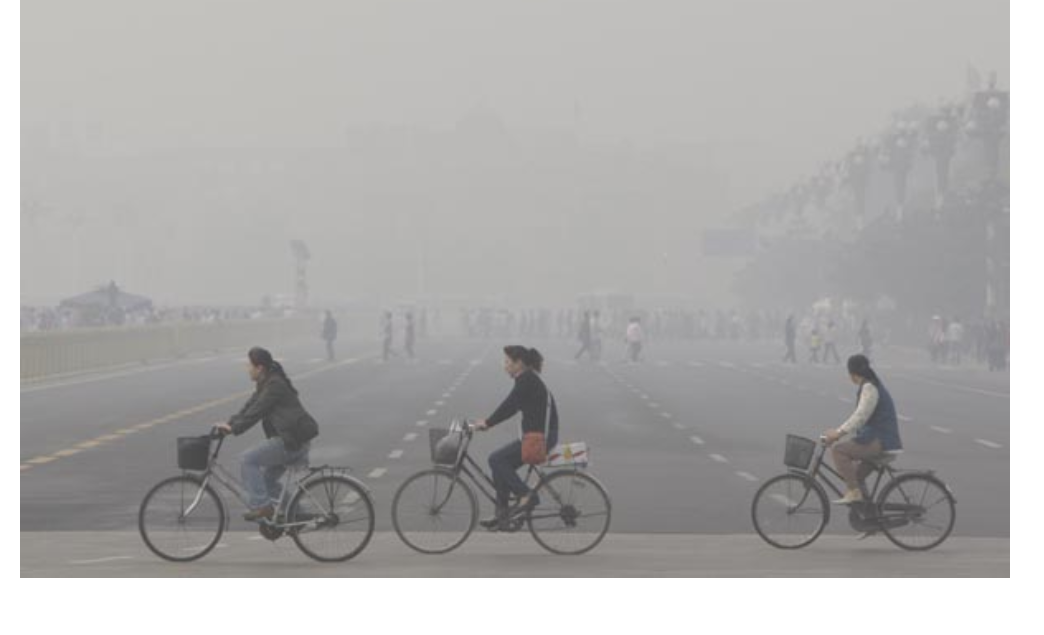
\includegraphics[width=0.82\linewidth]{img/di_fog.png}\end{center}
\ptesub{范文 Model Answer}
\begin{modelbox}
The following graph gives information about the view of a street in fog. This is a very dull picture taken in a fog, for a view of a street. According to this graph, at the central area, there are three bicycles ridden by women at the front and the color of them is black. You can see from this graph that, behind the bicycles, a white, thick blanket of fog covers a lot of people and street lights. What's more, in the background, four straight dashed lines lie on the road, and the color is white. Finally the weather is foggy and the sky is grey.
\end{modelbox}
\zh{下图给出的是大雾中一条街道的景象信息。这是一张在大雾中拍摄、画面非常昏暗的街景照片。根据该图，在中间区域有三辆自行车，骑车的都是女性且在最前面，车的颜色为黑色。从图中可以看到，在自行车后方，一层白色的浓雾笼罩着许多行人和路灯。此外，在背景中，路面上有四条笔直的白色虚线。最后，天气雾蒙蒙，天空呈灰色。}
\ptesub{你的作答（AI 语音识别逐词配色）}
\asrlegend
\begin{asrbox}
\sg{we} \sg{can} \sg{see} \sy{this} \sg{pictures} \sg{shows} \sg{sri} \sg{peoples} \sg{are} \sg{riding} \sg{their} \sg{bikes} \sg{and} \sg{some} \sg{people} \sg{are} \sg{working} \sg{and} \sr{in} \sy{this} \sg{ultimate} \sy{modified} \sy{atmosphere} \sg{is} \sg{not} \sg{good} \sg{and} \sg{we} \sg{cannot} \sg{see} \sg{many} \sy{things} \sg{in} \sg{this} \sg{picture}
\end{asrbox}
\smallskip
{\small\textbf{评分：}内容 \szero{0.6/5} \quad\textperiodcentered\quad 发音 \szero{10/90} \quad\textperiodcentered\quad 流利度 \szero{10/90}}\quad{\footnotesize\color{gray}（录音 0:34，用时 01:00）}
\end{qblock}

% ---------------- Q20 ----------------
\begin{qblock}{Q20\quad DI \#22\ \ Hospital Visits}{描述图 · 总分 \textcolor{cAccent}{\bfseries 25}/90}
\ptesub{配图 Image}
\begin{center}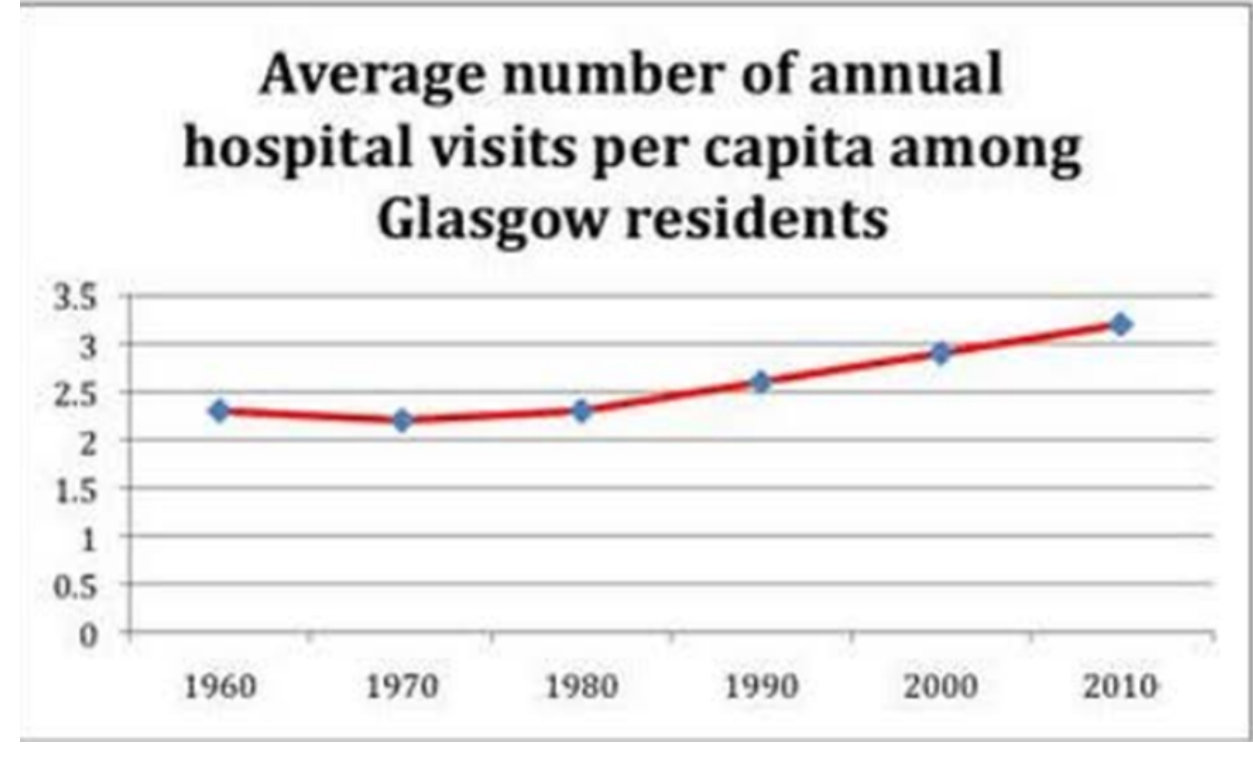
\includegraphics[width=0.85\linewidth]{img/di_hospital.png}\end{center}
\ptesub{范文 Model Answer}
\begin{modelbox}
The following graph gives information about the average number of annual hospital visits per capita among Glasgow residents. The horizontal axis is years, ranging from 1960 to 2010. According to this graph, in 1960, the value is around 2.5. And in 1970, the number is around 2. The highest one is around 3, which is in 2010. On the contrary, the lowest point is around 2, which is in 1970. In conclusion, if this trend continues, the average number of annual hospital visits will keep increasing in the future.
\end{modelbox}
\zh{下图给出的是格拉斯哥居民人均年度就医次数的信息。横轴是年份，从 1960 年到 2010 年。根据该图，1960 年数值约为 2.5；1970 年约为 2。最高点约为 3，出现在 2010 年；相反，最低点约为 2，出现在 1970 年。总之，如果这一趋势持续下去，未来人均年度就医次数将持续增加。}
\ptesub{你的作答（AI 语音识别逐词配色）}
\asrlegend
\begin{asrbox}
\sg{we} \sg{can} \sg{see} \sy{the} \sg{picture} \sg{shows} \sy{average} \sg{number} \sg{of} \sg{annual} \sg{hospital} \sg{visitors} \sg{per} \sg{capital} \sg{among} \sg{last} \sg{road} \sy{residents} \sg{and} \sg{the} \sg{people} \sg{about} \sy{this} \sg{is} \sy{a} \sg{become} \sg{more} \sg{and} \sg{more} \sg{and} \sg{until} \sg{twenty} \sg{one} \sg{twenty} \sg{ten} \sg{it} \sg{has} \sg{been} \sg{so} \sy{thirty} \sg{percent} \sg{of} \sg{it}
\end{asrbox}
\smallskip
{\small\textbf{评分：}内容 \spart{2/5} \quad\textperiodcentered\quad 发音 \spart{33/90} \quad\textperiodcentered\quad 流利度 \spart{20/90}}\quad{\footnotesize\color{gray}（录音 0:29，用时 00:55）}
\end{qblock}

% ---------------- Q21 ----------------
\begin{qblock}{Q21\quad DI \#74\ \ Majors' Number}{描述图 · 总分 \textcolor{cAccent}{\bfseries 65}/90}
\ptesub{配图 Image}
\begin{center}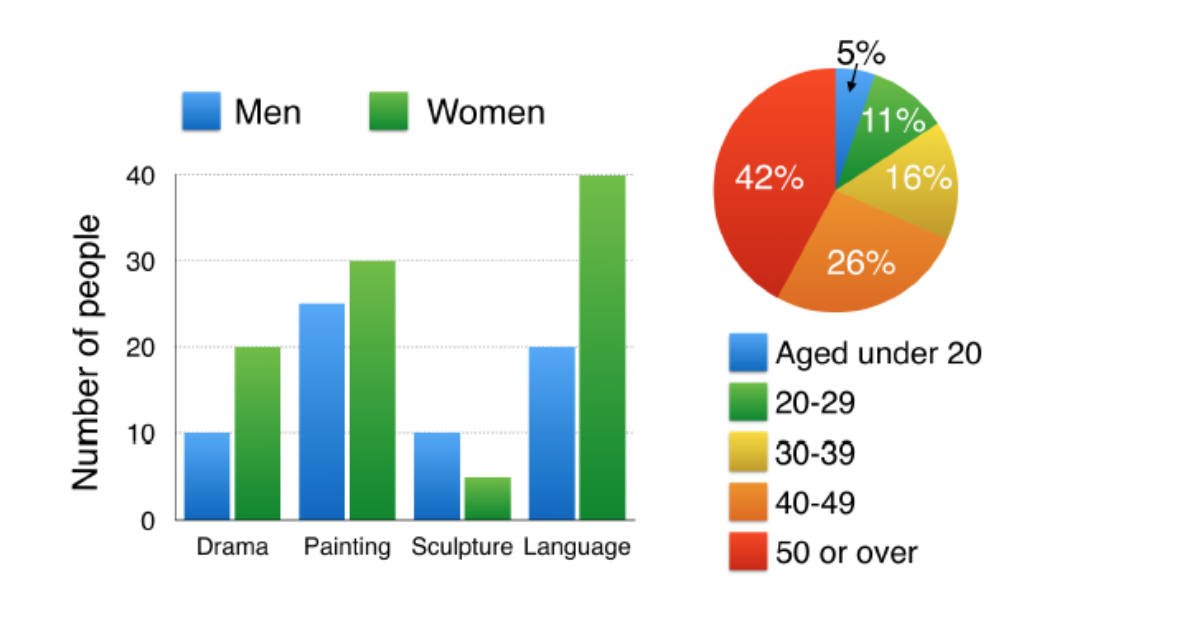
\includegraphics[width=0.97\linewidth]{img/di_majors.png}\end{center}
\ptesub{范文 Model Answer}
\begin{modelbox}
The following graph gives information about the major number. According to this graph, the highest number of people in the language is in women, around 40. On the contrary, the lowest number in painting is in men, which is around 20. And the largest proportion of the age composition is in age over 50, around 42\%. Finally, the smallest percentage is in age under 20, just 5. To sum up, this graph tells about men and women of different ages.
\end{modelbox}
\zh{下图给出的是各专业人数的信息。根据该图，语言专业人数最多的是女性，约为 40 人；相反，绘画专业人数最少的是男性，约为 20 人。年龄构成中占比最大的是 50 岁以上，约 42\%；占比最小的是 20 岁以下，仅 5\%。总而言之，该图讲述了不同年龄段男性和女性的情况。}
\ptesub{你的作答（AI 语音识别逐词配色）}
\asrlegend
\begin{asrbox}
\sg{we} \sg{can} \sg{see} \sy{the} \sg{chart} \sg{shows} \sg{number} \sg{of} \sg{people} \sg{in} \sy{drama} \sg{painting} \sg{sculpture} \sg{and} \sg{the} \sg{language} \sg{we} \sg{can} \sg{see} \sg{drama} \sg{and} \sg{painting} \sy{a} \sy{woman} \sg{become} \sg{more} \sg{and} \sy{the} \sg{sculpture} \sy{a} \sg{man} \sg{get} \sg{more} \sg{and} \sg{we} \sg{can} \sy{see} \sy{the} \sy{left} \sg{child} \sg{is} \sg{a} \sg{h} \sg{under} \sg{twenty} \sg{twenty} \sg{to} \sg{twenty} \sy{nine} \sg{or} \sy{the} \sg{fifty} \sg{or} \sg{over} \sg{and} \sg{fifty} \sg{or} \sg{over} \sy{cost} \sg{the} \sg{most}
\end{asrbox}
\smallskip
{\small\textbf{评分：}内容 \sfull{4.6/5} \quad\textperiodcentered\quad 发音 \sfull{78/90} \quad\textperiodcentered\quad 流利度 \spart{49/90}}\quad{\footnotesize\color{gray}（录音 0:36，用时 01:02）}
\end{qblock}


\ptetask{情景应答}{Respond to a Situation · RTS　Q22--24（评分含恰当性）}
% ---------------- Q22 ----------------
\begin{qblock}{Q22\quad RTS (C) \#26\ \ Checking Presentation Slides}{情景应答 · 总分 \textcolor{cAccent}{\bfseries 38}/90}
\ptesub{情景 Situation}
\begin{promptbox}
Your colleague asks if you can review the presentation slides they've prepared for an upcoming meeting. However, you realize you have several urgent tasks to complete by the end of the day. You need to politely ask for more time to ensure you can give their slides the attention they deserve. What would you say to your colleague?
\end{promptbox}
\zh{你的同事问你能否帮忙看一下他为即将到来的会议准备的演示幻灯片。然而你意识到自己当天还有几项紧急任务要在下班前完成。你需要礼貌地请求多给你一些时间，以确保能认真对待他的幻灯片。你会对同事说什么？}
\ptesub{参考答案 Model Answer}
\begin{modelbox}
Hey, I appreciate you reaching out about the presentation slides. But I have a few urgent tasks to attend to today, so I may not be able to review them thoroughly right away. Would it be possible to have until tomorrow morning to give them a proper look? I want to ensure I can provide valuable feedback. Thanks for understanding!
\end{modelbox}
\zh{嘿，谢谢你来找我看演示幻灯片。不过我今天还有几项紧急任务要处理，所以可能没法马上仔细看。能不能给我到明天早上的时间，让我好好看一看？我想确保能给出有价值的反馈。谢谢你的理解！}
\ptesub{你的作答（AI 语音识别逐词配色）}
\asrlegend
\begin{asrbox}
\sy{hi} \sg{i} \sg{know} \sg{you} \sg{want} \sg{to} \sg{ask} \sg{me} \sg{if} \sg{i} \sg{can} \sg{review} \sg{the} \sg{presentation} \sg{slide} \sg{you} \sg{have} \sy{prepared} \sg{for} \sg{an} \sy{oncoming} \sg{meeting} \sg{but} \sg{however} \sg{i} \sg{realize} \sg{i} \sg{have} \sg{several} \sr{arjun} \sg{test} \sg{to} \sg{complete} \sg{by} \sy{the} \sg{end} \sg{of} \sg{day} \sg{so} \sg{i} \sg{need} \sy{to} \sg{politely} \sg{ask} \sg{for} \sg{more} \sg{time} \sg{to} \sg{ensure} \sg{i} \sg{can} \sg{give} \sg{your} \sg{slide} \sg{and} \sy{attend} \sg{your} \sg{deserve} \sg{so} \sg{please} \sg{give} \sg{me} \sg{the} \sg{time}
\end{asrbox}
\smallskip
{\small\textbf{评分：}恰当性 \spart{53/90} \quad\textperiodcentered\quad 发音 \spart{28/90} \quad\textperiodcentered\quad 流利度 \spart{39/90}}\quad{\footnotesize\color{gray}（录音 0:40，用时 01:30）}
\end{qblock}

% ---------------- Q23 ----------------
\begin{qblock}{Q23\quad RTS (C) \#27\ \ Feasible Options}{情景应答 · 总分 \textcolor{cAccent}{\bfseries 44}/90}
\ptesub{情景 Situation}
\begin{promptbox}
You're planning a weekend getaway with friends, and they're discussing the activities they want to do. However, you realize some of the suggestions might not be feasible due to time constraints or budget limitations. You need to gently guide the conversation towards more realistic options without dampening the excitement. What would you say to your friends?
\end{promptbox}
\zh{你正和朋友们计划一次周末短途出游，他们在讨论想做的各种活动。然而你意识到，由于时间或预算限制，有些建议可能不太可行。你需要在不打击大家热情的前提下，温和地把话题引向更现实的选择。你会对朋友们说什么？}
\ptesub{参考答案 Model Answer}
\begin{modelbox}
Hey everyone, I'm loving all the ideas for our weekend getaway! Just a heads up, I think some of the activities might be a bit tricky to fit into our schedule or budget. How about we brainstorm some alternative options that are more practical but still super fun? We want to make the most of our time together without stressing about logistics. Let's keep the excitement going and find the perfect balance of adventure and affordability!
\end{modelbox}
\zh{嘿，各位，我很喜欢大家为周末出游想到的所有点子！不过提醒一下，我觉得有些活动可能不太好安排进我们的日程或预算。不如我们一起头脑风暴一些更实际但同样超有趣的备选方案？我们想充分利用在一起的时间，而不必为各种安排操心。让我们保持这份兴奋，找到冒险与实惠之间的完美平衡吧！}
\ptesub{你的作答（AI 语音识别逐词配色）}
\asrlegend
\begin{asrbox}
\sy{hi} \sg{i} \sg{notice} \sy{that} \sg{you} \sg{are} \sg{discussing} \sy{the} \sg{activity} \sy{you} \sg{want} \sg{to} \sg{do} \sg{however} \sg{i} \sy{realize} \sg{some} \sg{of} \sg{suggestions} \sg{might} \sr{not} \sg{be} \sg{feasible} \sg{to} \sg{choose} \sg{time} \sg{contrast} \sg{or} \sg{budget} \sg{limitation} \sg{so} \sg{i} \sg{think} \sg{i} \sg{need} \sg{to} \sg{gently} \sy{guides} \sg{the} \sg{conversation} \sr{holds} \sg{more} \sg{relaxed} \sr{iq} \sg{options} \sg{without} \sr{damaging} \sg{the} \sg{excitement} \sg{um} \sg{let's} \sg{let's} \sg{have} \sg{a} \sg{talk}
\end{asrbox}
\smallskip
{\small\textbf{评分：}恰当性 \spart{59/90} \quad\textperiodcentered\quad 发音 \spart{40/90} \quad\textperiodcentered\quad 流利度 \spart{40/90}}\quad{\footnotesize\color{gray}（录音 0:40，用时 01:32）}
\end{qblock}

% ---------------- Q24 ----------------
\begin{qblock}{Q24\quad RTS (C) \#28\ \ Food Choice}{情景应答 · 总分 \textcolor{cAccent}{\bfseries 54}/90}
\ptesub{情景 Situation}
\begin{promptbox}
You're hosting a dinner party for friends, and they're suggesting elaborate dishes that require a lot of preparation. However, you realize you have limited time and resources to cook such elaborate meals. You need to gently steer the conversation towards simpler, yet equally delicious. What would you say to your friends?
\end{promptbox}
\zh{你正在为朋友们举办一场晚餐聚会，他们建议做一些需要大量准备工作的精致菜肴。然而你意识到自己时间和资源有限，没法做这么复杂的大餐。你需要温和地把话题引向更简单却同样美味的选择。你会对朋友们说什么？}
\ptesub{参考答案 Model Answer}
\begin{modelbox}
Hey everyone, I'm excited about our dinner party! Some of the dishes suggested sound amazing, but I'm worried they might be too time-consuming given my schedule. How about we focus on simpler recipes that still pack a punch in flavor? Maybe we can opt for some crowd-pleasers like pasta dishes, grilled meats, or hearty salads that are easy to prepare but still delicious. Let's keep it stress-free and enjoyable for everyone!
\end{modelbox}
\zh{嘿，各位，我对我们的晚餐聚会很期待！有些建议的菜听起来棒极了，但我担心考虑到我的时间安排，它们可能太费工夫了。不如我们专注于一些更简单、但味道依然十足的食谱？也许可以选一些大众喜爱的菜，比如意面、烤肉或丰盛的沙拉，它们做起来简单又好吃。让我们把它办得轻松又愉快吧！}
\ptesub{你的作答（AI 语音识别逐词配色）}
\asrlegend
\begin{asrbox}
\sy{hi} \sg{i} \sg{notice} \sy{that} \sg{you're} \sg{suggestion} \sy{elaborate} \sg{dishes} \sy{that} \sg{require} \sg{a} \sg{lot} \sg{of} \sy{proper} \sg{preparation} \sg{however} \sg{i} \sg{realize} \sg{we} \sg{have} \sy{limited} \sg{time} \sg{and} \sg{resources} \sg{to} \sg{cook} \sg{such} \sy{elaborate} \sg{meals} \sg{so} \sg{i} \sg{think} \sg{we} \sg{should} \sr{think} \sy{a} \sg{generally} \sr{steer} \sg{the} \sg{conversation} \sy{towards} \sg{simpler} \sg{yes} \sy{the} \sr{equal} \sg{delicious} \sg{so} \sg{let's} \sg{have} \sg{a} \sg{talk}
\end{asrbox}
\smallskip
{\small\textbf{评分：}恰当性 \sfull{69/90} \quad\textperiodcentered\quad 发音 \spart{52/90} \quad\textperiodcentered\quad 流利度 \spart{48/90}}\quad{\footnotesize\color{gray}（录音 0:40，用时 01:31）}
\end{qblock}


\ptetask{简短回答}{Answer Short Question · ASQ　Q25--30（单题 0/1）}
\begin{notebox}
{\footnotesize\color{gray}ASQ 考查“听问答词”，单题 0/1。你的录音不收；下表为题目、中文翻译与参考答案（绿）。}
\smallskip\par
\textbf{Q25\quad ASQ \#1358}\quad{\footnotesize\color{gray}（用时 00:19，得分 \sfull{1/1}）}\\
Which is the biggest one, the elephant, the tiger, or the cheetah?\\
\zh{大象、老虎和猎豹，哪一个最大？}\\
参考答案：{\color{cFix}\textbf{Elephant}}（大象）
\par\smallskip
\textbf{Q26\quad ASQ \#1335}\quad{\footnotesize\color{gray}（用时 00:17，得分 \szero{0/1}）}\\
How do we call a person who is about the same age?\\
\zh{我们怎么称呼一个年龄相仿的人？}\\
参考答案：{\color{cFix}\textbf{Contemporary / peer}}（同龄人 / 同辈人）
\par\smallskip
\textbf{Q27\quad ASQ \#1359}\quad{\footnotesize\color{gray}（用时 00:16，得分 \szero{0/1}）}\\
What is the top surface inside the room?\\
\zh{房间内部最上面的那个面叫什么？}\\
参考答案：{\color{cFix}\textbf{Ceiling}}（天花板）
\par\smallskip
\textbf{Q28\quad ASQ \#1376}\quad{\footnotesize\color{gray}（用时 00:17，得分 \szero{0/1}）}\\
What do we call a person who studies mystery?\\
\zh{我们怎么称呼研究神秘事物的人？}\\
参考答案：{\color{cFix}\textbf{Mystic / occult}}（神秘主义者 / 玄学）
\par\smallskip
\textbf{Q29\quad ASQ \#1375}\quad{\footnotesize\color{gray}（用时 00:20，得分 \szero{0/1}）}\\
What do we call the event in which people move through a public place to celebrate an important day or event?\\
\zh{我们把人们穿过公共场所以庆祝重要日子或事件的活动叫什么？}\\
参考答案：{\color{cFix}\textbf{Parade}}（游行）
\par\smallskip
\textbf{Q30\quad ASQ \#1377}\quad{\footnotesize\color{gray}（用时 00:15，得分 \szero{0/1}）}\\
What do we call a diagram in which an object would appear to viewers if it were cut from top to bottom?\\
\zh{把物体从上到下剖开后呈现给观者的图叫什么？}\\
参考答案：{\color{cFix}\textbf{Section}}（剖面图 / 截面）
\end{notebox}

\end{document}
